% Options for packages loaded elsewhere
\PassOptionsToPackage{unicode}{hyperref}
\PassOptionsToPackage{hyphens}{url}
\documentclass[
  11pt,
]{article}
\usepackage{xcolor}
\usepackage[left=2.2cm,right=2.2cm,top=1.8cm,bottom=1.8cm]{geometry}
\usepackage{amsmath,amssymb}
\setcounter{secnumdepth}{5}
\usepackage{iftex}
\ifPDFTeX
  \usepackage[T1]{fontenc}
  \usepackage[utf8]{inputenc}
  \usepackage{textcomp} % provide euro and other symbols
\else % if luatex or xetex
  \usepackage{unicode-math} % this also loads fontspec
  \defaultfontfeatures{Scale=MatchLowercase}
  \defaultfontfeatures[\rmfamily]{Ligatures=TeX,Scale=1}
\fi
\usepackage{lmodern}
\ifPDFTeX\else
  % xetex/luatex font selection
\fi
% Use upquote if available, for straight quotes in verbatim environments
\IfFileExists{upquote.sty}{\usepackage{upquote}}{}
\IfFileExists{microtype.sty}{% use microtype if available
  \usepackage[]{microtype}
  \UseMicrotypeSet[protrusion]{basicmath} % disable protrusion for tt fonts
}{}
\makeatletter
\@ifundefined{KOMAClassName}{% if non-KOMA class
  \IfFileExists{parskip.sty}{%
    \usepackage{parskip}
  }{% else
    \setlength{\parindent}{0pt}
    \setlength{\parskip}{6pt plus 2pt minus 1pt}}
}{% if KOMA class
  \KOMAoptions{parskip=half}}
\makeatother
\usepackage{longtable,booktabs,array}
\usepackage{caption}
\captionsetup[table]{skip=6pt}
\newcounter{none} % for unnumbered tables
\usepackage{calc} % for calculating minipage widths
% Correct order of tables after \paragraph or \subparagraph
\usepackage{etoolbox}
\makeatletter
\patchcmd\longtable{\par}{\if@noskipsec\mbox{}\fi\par}{}{}
\makeatother
% Allow footnotes in longtable head/foot
\IfFileExists{footnotehyper.sty}{\usepackage{footnotehyper}}{\usepackage{footnote}}
\makesavenoteenv{longtable}
\usepackage{graphicx}
\makeatletter
\newsavebox\pandoc@box
\newcommand*\pandocbounded[1]{% scales image to fit in text height/width
  \sbox\pandoc@box{#1}%
  \Gscale@div\@tempa{\textheight}{\dimexpr\ht\pandoc@box+\dp\pandoc@box\relax}%
  \Gscale@div\@tempb{\linewidth}{\wd\pandoc@box}%
  \ifdim\@tempb\p@<\@tempa\p@\let\@tempa\@tempb\fi% select the smaller of both
  \ifdim\@tempa\p@<\p@\scalebox{\@tempa}{\usebox\pandoc@box}%
  \else\usebox{\pandoc@box}%
  \fi%
}
% Set default figure placement to htbp
\def\fps@figure{htbp}
\makeatother
% definitions for citeproc citations
\NewDocumentCommand\citeproctext{}{}
\NewDocumentCommand\citeproc{mm}{%
  \begingroup\def\citeproctext{#2}\cite{#1}\endgroup}
\makeatletter
 % allow citations to break across lines
 \let\@cite@ofmt\@firstofone
 % avoid brackets around text for \cite:
 \def\@biblabel#1{}
 \def\@cite#1#2{{#1\if@tempswa , #2\fi}}
\makeatother
\newlength{\cslhangindent}
\setlength{\cslhangindent}{1.5em}
\newlength{\csllabelwidth}
\setlength{\csllabelwidth}{3em}
\newenvironment{CSLReferences}[2] % #1 hanging-indent, #2 entry-spacing
 {\begin{list}{}{%
  \setlength{\itemindent}{0pt}
  \setlength{\leftmargin}{0pt}
  \setlength{\parsep}{0pt}
  % turn on hanging indent if param 1 is 1
  \ifodd #1
   \setlength{\leftmargin}{\cslhangindent}
   \setlength{\itemindent}{-1\cslhangindent}
  \fi
  % set entry spacing
  \setlength{\itemsep}{#2\baselineskip}}}
 {\end{list}}
\usepackage{calc}
\newcommand{\CSLBlock}[1]{\hfill\break\parbox[t]{\linewidth}{\strut\ignorespaces#1\strut}}
\newcommand{\CSLLeftMargin}[1]{\parbox[t]{\csllabelwidth}{\strut#1\strut}}
\newcommand{\CSLRightInline}[1]{\parbox[t]{\linewidth - \csllabelwidth}{\strut#1\strut}}
\newcommand{\CSLIndent}[1]{\hspace{\cslhangindent}#1}
\setlength{\emergencystretch}{3em} % prevent overfull lines
\providecommand{\tightlist}{%
  \setlength{\itemsep}{0pt}\setlength{\parskip}{0pt}}
% Three-part paragraph scaffolding for manuscript revision.
%
% bullets  -- boiled-down topic sentence + bullet points
%             small, sans-serif, dark gray; paragraph number [N] prepended
% rgt      -- author's rewrite (initially a placeholder)
%             small, italic, dark blue
% orig     -- original Claude-authored draft
%             normal size, light gray
%
% Presentation order per paragraph: bullets -> rgt -> orig
% Strip with: strip-claudecode -i report.Rmd

\usepackage{xcolor}

\newcounter{pgraph}

\newenvironment{bullets}{%
  \stepcounter{pgraph}%
  \begin{quote}\small\sffamily\color[gray]{0.30}%
  {\normalfont\scriptsize\color[gray]{0.58}[\thepgraph]\enspace}}{%
  \end{quote}}

\newenvironment{rgt}{%
  \begin{quote}\small\itshape\color[RGB]{20,60,160}}{%
  \end{quote}}

\newenvironment{orig}{%
  \begin{quote}\normalsize\color[gray]{0.55}}{%
  \end{quote}}

% backward compat alias
\newenvironment{claudecode}{\begin{orig}}{\end{orig}}
\usepackage{amsmath}
\usepackage{amssymb}
\usepackage{setspace}
\setstretch{1.0}
\usepackage{booktabs}
\usepackage{longtable}
\usepackage{array}
\usepackage{multirow}
\usepackage{wrapfig}
\usepackage{float}
\usepackage{colortbl}
\usepackage{pdflscape}
\usepackage{tabu}
\usepackage{threeparttable}
\usepackage{threeparttablex}
\usepackage[normalem]{ulem}
\usepackage{makecell}
\usepackage{xcolor}
\usepackage{bookmark}
\IfFileExists{xurl.sty}{\usepackage{xurl}}{} % add URL line breaks if available
\urlstyle{same}
% fallback for those not using the hyperref driver hyperxmp:
\makeatletter
\@ifundefined{xmpquote}{\newcommand{\xmpquote}[1]{#1}}{}
\makeatother
\hypersetup{
  pdftitle={Exposure-weighted versus lagged-treatment carryover specifications under differential-correlation biomarker interactions: a factorial simulation study},
  pdfauthor={pmsimstats team},
  hidelinks,
  pdfcreator={LaTeX via pandoc}}

\title{Exposure-weighted versus lagged-treatment carryover specifications under differential-correlation biomarker interactions: a factorial simulation study}
\author{pmsimstats team}
\date{2026-07-30}

\begin{document}
\maketitle

\section*{Abstract}\label{abstract}
\addcontentsline{toc}{section}{Abstract}

\textbf{Background.} Aggregated N-of-1 trials pool repeated within-patient
on/off contrasts to validate predictive biomarkers. Under the
multivariate-normal (MVN) differential-correlation architecture
(Architecture B), in which the biomarker-treatment interaction is
encoded in a treatment-state-dependent correlation, a companion study
found that carryover -- residual drug effect that decays after
discontinuation -- costs up to roughly 31\% of power in relative
terms. The analyst must still decide how to represent residual
exposure in the linear predictor, and it is not established which
representation is most robust to the (typically unknown)
pharmacokinetic decay shape.

\textbf{Methods.} We compare two analysis-model specifications for the
drug-exposure regressor under Architecture B: an exposure-weighted
continuous indicator that assumes a parametric decay and half-life
(M2, the current default), and the binary on-drug indicator augmented
by a lagged just-off-drug term that estimates carryover
non-parametrically (M3, the classical crossover device). We embed
them in an ADEMP-structured factorial simulation\textsuperscript{\citeproc{ref-morris2019simulation}{1}} crossing two data-generating process (DGP)
decay forms (exponential, Weibull) with the two specifications, under
three trial designs, two sample sizes, and three interaction
strengths (216 cells, 500 replicates each), plus four single-axis
sensitivity blocks and a cluster-robust recalibration. Every
performance measure is reported with its Monte Carlo standard error
(MCSE).

\textbf{Results.} M2 attains the highest power only in the two designs
with a blinded-discontinuation phase (Hybrid and OL+BDC), where its
advantage over M3 is about 10 percentage points (0.860 vs 0.770 at
the reference cell). Under the classical crossover (CO) design M2 is
markedly inferior (0.488 vs 0.830 for M3, which tracks the binary
indicator closely). Where M2 leads, the lead is robust to decay-shape
and half-life mis-specification and to autocorrelation strength, and
a paired-McNemar high-precision rerun confirms it is real at the
highest-leverage cell (\(+7.2\) points, \(p = 1.2 \times 10^{-7}\)),
though the two specifications are statistically tied at three of
four other rerun cells. The model-based interaction test is mildly
conservative (mean null rejection 0.039), an artifact of the working
covariance that a CR2 cluster-robust standard error removes without
disturbing the ranking.

\textbf{Conclusions.} Under Architecture B, the exposure-weighted
predictor M2, reported with a cluster-robust standard error, is
recommended for the Hybrid and OL+BDC designs; the lagged-treatment
specification M3 is preferable, or at least not worse, under a
crossover design. Across all conditions, anticipated dropout governs
power far more than the choice between the two specifications, and
should dominate design effort accordingly. This manuscript restricts
the grid to Architecture B and to the exponential and Weibull decay
forms, and does not evaluate the binary on-drug specification (M1)
or Architecture A (mean moderation); the full-scope evaluation,
including those comparisons, is in the companion report.Rmd /
report-slim.Rmd manuscripts.

\section{Introduction}\label{introduction}

\subsection{A short primer on aggregated N-of-1 trials}\label{a-short-primer-on-aggregated-n-of-1-trials}

\begin{bullets}

\textbf{Aggregated N-of-1 trials pool repeated within-patient on/off
contrasts to validate predictive biomarkers at far smaller sample
sizes than parallel-group trials.}

\begin{itemize}\setlength{\itemsep}{2pt}\setlength{\parskip}{0pt}
\item A single N-of-1 trial crosses one patient on and off treatment
repeatedly; pooling many such series gives population-level
inference.
\item The estimand is the biomarker-treatment interaction: whether a
baseline covariate $B_i$ modifies the treatment effect.
\item Three designs (crossover (CO); open-label plus
blinded-discontinuation (OL+BDC); Hybrid) differ in how on- and
off-drug occasions are arranged.
\end{itemize}

\end{bullets}

\begin{rgt}
rgt to complete.

\end{rgt}

\begin{orig}
In a single N-of-1 trial one patient is repeatedly crossed between
active treatment and a comparator over a sequence of measurement
occasions; the within-patient on-versus-off contrast estimates that
patient's individual treatment effect. An \emph{aggregated} N-of-1 trial
pools many such single-patient series in a mixed model, trading some
within-patient resolution for population-level inference and far
smaller sample sizes than a parallel-group trial\textsuperscript{\citeproc{ref-hendrickson2020}{2}}. The estimand of interest is the
biomarker-treatment interaction, i.e.~whether a baseline covariate
\(B_i\) modifies the treatment effect. We study three designs that
differ in how on- and off-drug occasions are arranged: a classical
crossover (CO), an open-label plus blinded-discontinuation design
(OL+BDC), and a Hybrid N-of-1 design; these are defined in §3.

\end{orig}

\begin{bullets}

\textbf{Carryover -- residual drug effect that decays after
discontinuation -- contaminates off-drug occasions and attenuates
the interaction test.}

\begin{itemize}\setlength{\itemsep}{2pt}\setlength{\parskip}{0pt}
\item The drug effect fades over days to weeks rather than switching
off, so off-drug occasions carry residual exposure.
\item Treating them as cleanly off-drug mis-specifies the design
matrix.
\item We ask which of two analyst-side exposure representations is
most robust to the resulting attenuation.
\end{itemize}

\end{bullets}

\begin{rgt}
rgt to complete.

\end{rgt}

\begin{orig}
The inferential nuisance specific to this setting is \textbf{carryover}.
When the drug is discontinued its pharmacological effect does not
switch off but decays over days to weeks, so off-drug occasions
carry residual exposure. Treating them as cleanly off-drug
mis-specifies the design matrix and attenuates the interaction test.
The question we take up is which of two analyst-side representations
of residual exposure best recovers the lost power.

\end{orig}

\subsection{What is already known, and the gap}\label{what-is-already-known-and-the-gap}

\begin{bullets}

\textbf{Under the differential-correlation architecture (B), carryover
costs roughly 31\% of power in relative terms, and the choice of
analysis specification for representing residual exposure has not
been evaluated against decay-form uncertainty.}

\begin{itemize}\setlength{\itemsep}{2pt}\setlength{\parskip}{0pt}
\item Architecture B encodes the biomarker interaction in a
treatment-state-dependent correlation, which carryover erodes
directly.
\item A companion study fixed the decay shape at exponential and
used a single analysis specification.
\item This manuscript restricts to Architecture B, where the
carryover problem is largest, and asks which specification is most
robust when the decay shape is uncertain.
\end{itemize}

\end{bullets}

\begin{rgt}
rgt to complete.

\end{rgt}

\begin{orig}
A companion paper\textsuperscript{\citeproc{ref-pmsimstats_dgp_architectures2026}{3}}, extending
Hendrickson\textsuperscript{\citeproc{ref-hendrickson2020}{2}}, shows that under \textbf{Architecture B}
(multivariate-normal differential correlation) the interaction lives
in the treatment-state-dependent covariance
\(\text{Cor}(B_i, BR_{it}) = c_{bm} \cdot \phi(t_{sd})\), which
carryover erodes directly: at a half-life of one week, power falls
by up to roughly 31\% in relative terms, strongly design-dependent
(largest under OL+BDC, negligible under CO). Under the alternative
Architecture A (direct mean moderation), the corresponding loss is
only 1-3\%; that architecture, and the third combined Architecture C,
are outside the scope of this manuscript, which restricts to
Architecture B, the architecture in which the carryover problem is
largest and in which Hendrickson's original results were obtained.
That companion work, however, fixed the decay shape at exponential
and evaluated a single analysis-model specification throughout,
leaving open which analyst-side representation of residual exposure
is most robust when the true decay shape is uncertain.

\end{orig}

\subsection{This paper}\label{this-paper}

\begin{bullets}

\textbf{We compare two analyst-side exposure representations --
exposure-weighted (M2) and lagged-treatment (M3) -- across decay
forms under Architecture B.}

\begin{itemize}\setlength{\itemsep}{2pt}\setlength{\parskip}{0pt}
\item M2 commits to a parametric decay and half-life; M3 estimates
carryover non-parametrically via a lagged term.
\item Each is crossed against exponential and Weibull DGP decay
forms.
\item The question is whether one specification is recommendable or
the choice is design-dependent.
\end{itemize}

\end{bullets}

\begin{rgt}
rgt to complete.

\end{rgt}

\begin{orig}
We evaluate two analyst-side representations of drug exposure in the
linear predictor: an exposure-weighted continuous indicator that
commits to a parametric decay form and half-life (\textbf{M2}, the
current default), and the binary on-drug indicator augmented by a
lagged just-off-drug term that estimates carryover non-parametrically
(\textbf{M3}, the classical crossover device of Jones and Kenward\textsuperscript{\citeproc{ref-jones2014crossover}{4}}). We cross these against the exponential and
Weibull data-generating decay forms and ask whether a single
specification can be recommended or whether the choice is
design-dependent. The study follows the ADEMP reporting framework of
Morris, White, and Crowther\textsuperscript{\citeproc{ref-morris2019simulation}{1}}, with every
performance measure accompanied by its MCSE. Section 3 gives the
simulation design in ADEMP order; Section 4 the results; Section 5
the practical implications for trialists.

\end{orig}

\section{Simulation design}\label{simulation-design}

\subsection{Aims}\label{aims}

\begin{bullets}

\textbf{The aim is to identify, under Architecture B, which of M2 and
M3 is the more robust carryover-mitigation strategy across DGP decay
forms and trial designs.}

\begin{itemize}\setlength{\itemsep}{2pt}\setlength{\parskip}{0pt}
\item Quantify the power cost of analysis-model carryover
mis-specification under Architecture B.
\item Identify which of M2 and M3 is more robust across the DGP
decay-form grid and across trial designs.
\item Verify whether the ranking survives half-life mis-specification
and other single-axis perturbations (Tier 2).
\end{itemize}

\end{bullets}

\begin{rgt}
rgt to complete.

\end{rgt}

\begin{orig}
The aim of this study is to quantify, under Architecture B, the cost
of analysis-model carryover mis-specification in aggregated N-of-1
and crossover trials, and to identify which of the two
carryover-mitigation strategies, M2 or M3, is more robust across the
DGP decay-form grid and across trial designs. A secondary aim,
addressed in the Tier 2 sensitivity blocks, is to verify that the
ranking survives perturbation of autocorrelation strength, dropout,
half-life mis-specification, and interaction effect size.

\end{orig}

\subsection{Data-generating mechanism}\label{data-generating-mechanism}

\begin{bullets}

\textbf{This manuscript retains only Architecture B (MVN differential
correlation); the biomarker and biological response are jointly MVN
with correlation decaying off-drug.}

\begin{itemize}\setlength{\itemsep}{2pt}\setlength{\parskip}{0pt}
\item $\text{Cor}(B_i, BR_{it}) = c_{bm}\,\phi(t_{sd})$, where $\phi$
is the decay form.
\item Architecture A (mean moderation) and the combined Architecture
C are out of scope here; see report.Rmd for the cross-architecture
comparison.
\item Two decay forms for $\phi$ are evaluated: exponential and
Weibull. The linear form is dropped from this manuscript's scope.
\end{itemize}

\end{bullets}

\begin{rgt}
rgt to complete.

\end{rgt}

\begin{orig}
In Architecture B, the biomarker and biological response are jointly
drawn from a multivariate normal with treatment-state-dependent
correlation
\(\text{Cor}(B_i, BR_{it}) = c_{bm} \cdot \phi(t_{sd})\), where \(\phi\)
is the decay form and \(t_{sd}\) is time since drug discontinuation.
Architecture A (direct mean moderation) and the combined Architecture
C are outside the scope of this manuscript; the full grid comparison
across architectures is reported in the companion report.Rmd /
report-slim.Rmd manuscripts. In both architectures the decay function
\(\phi : \mathbb{R}_+ \to [0, 1]\) maps \(t_{sd}\) to a residual-effect
multiplier. We evaluate two forms here, each parameterized to match
a common half-life \(t_{1/2}\); the linear form used in the full-scope
manuscripts is dropped from this narrower evaluation.

\end{orig}

\subsubsection{Exponential decay}\label{exponential-decay}

\[
\phi_{\text{exp}}(t_{sd}) =
  \exp\left(-\lambda t_{sd}\right), \qquad
  \lambda = \frac{\ln 2}{t_{1/2}}
\]

\begin{bullets}

\textbf{The exponential form is the natural reference decay because
it corresponds to first-order elimination kinetics.}

\begin{itemize}\setlength{\itemsep}{2pt}\setlength{\parskip}{0pt}
\item Used throughout the companion manuscript and implemented in
\texttt{implementations/tidyverse/R/functions.R}.
\item Corresponds to classical pharmacokinetic first-order
elimination.
\item Retained as the reference against which the Weibull form is
compared.
\end{itemize}

\end{bullets}

\begin{rgt}
rgt to complete.

\end{rgt}

\begin{orig}
This is the form used throughout the companion manuscript and
currently implemented in \texttt{implementations/tidyverse/R/functions.R}.
It corresponds to first-order elimination kinetics and is the
default assumption in classical pharmacokinetics; we retain it here
as the natural reference against which the Weibull form is compared.

\end{orig}

\subsubsection{Weibull decay}\label{weibull-decay}

\[
\phi_{\text{weib}}(t_{sd}) =
  \exp\left(-\left(\lambda_w t_{sd}\right)^{k}\right), \qquad
  \lambda_w = \frac{(\ln 2)^{1/k}}{t_{1/2}}
\]

\begin{bullets}

\textbf{The Weibull shape parameter $k$ controls whether the
elimination tail is heavier or lighter than exponential.}

\begin{itemize}\setlength{\itemsep}{2pt}\setlength{\parskip}{0pt}
\item $k < 1$: slower elimination with a prolonged low-concentration
tail (evaluated at $k = 0.7$).
\item $k > 1$: accelerated off-drug clearance via saturable clearance
or active-transporter kinetics (evaluated at $k = 1.5$).
\item $k = 1$ recovers the exponential form exactly.
\end{itemize}

\end{bullets}

\begin{rgt}
rgt to complete.

\end{rgt}

\begin{orig}
A shape parameter \(k\) governs whether the elimination tail is
heavier (\(k < 1\), slow elimination) or lighter (\(k > 1\), accelerated
off-drug clearance) than the exponential, which is recovered exactly
at \(k = 1\). We report results at \(k = 0.7\), representing a drug with
a prolonged low-concentration tail, and at \(k = 1.5\), which captures
drugs with saturable clearance or active-transporter kinetics.
Together with \(k = 1.0\) (numerically identical to the exponential
form), this yields four decay-shape levels in the grid.

\end{orig}

\subsection{Estimand and analysis specifications}\label{estimand-and-analysis-specifications}

\begin{bullets}

\textbf{The estimand is the on-drug biomarker-response correlation
$c_{bm}$; the null estimand $c_{bm} = 0$ is the Type I error row.}

\begin{itemize}\setlength{\itemsep}{2pt}\setlength{\parskip}{0pt}
\item Under Architecture B the interaction estimand is $c_{bm}$,
dimensionless.
\item Bias, empirical SE, and MSE are reported on the calibrated
effect-size scale defined in \texttt{docs/19}.
\item The null estimand for Type I verification is the $c_{bm} = 0$
row of the grid.
\end{itemize}

\end{bullets}

\begin{rgt}
rgt to complete.

\end{rgt}

\begin{orig}
Under Architecture B, the interaction estimand is the on-drug
biomarker-response correlation \(c_{bm}\), dimensionless. Bias and
empirical standard error are reported on the calibrated effect-size
scale (expected on-drug response difference per SD of biomarker at
\(t_{1/2} = 0\)) defined in
\texttt{docs/19-mean-moderation-implementation-notes.tex}; power and Type I
error are reported on the native test-statistic scale. The null
estimand for Type I error verification is \(c_{bm} = 0\), realized by
the \(c_{bm} = 0\) row of the parameter grid.

\end{orig}

The analysis model is \texttt{nlme::lme(Sx\ \textasciitilde{}\ bm\ *\ X\ +\ t,\ random\ =\ \textasciitilde{}1\ \textbar{}\ ptID,\ correlation\ =\ corCAR1(form\ =\ \textasciitilde{}\ t\ \textbar{}\ ptID))} for both
specifications. They differ only in the drug exposure predictor \(X\).

\subsubsection{M2: exposure-weighted (continuous predictor)}\label{m2-exposure-weighted-continuous-predictor}

\begin{bullets}

\textbf{M2 uses a continuous exposure-weighted predictor that
commits to a specific decay form and half-life, and is the current
pmsimstats-ng default.}

\begin{itemize}\setlength{\itemsep}{2pt}\setlength{\parskip}{0pt}
\item $X = \text{Dbc}_{it}$: decays off-drug according to the
analyst's assumed form and half-life.
\item Well-matched when the analyst's assumed form coincides with
the true DGP form; mis-specified otherwise.
\item Sensitivity of M2 to assumed-versus-true mismatch is evaluated
in Tier 2 block S2.
\end{itemize}

\end{bullets}

\begin{rgt}
rgt to complete.

\end{rgt}

\begin{orig}
\(X = \text{Dbc}_{it}\), the continuous exposure-decayed predictor
constructed to match the analyst's assumed decay form and half-life.
This is the current pmsimstats-ng default specification. At on-drug
timepoints \(D_{bc,it} = 1\) regardless of the assumed half-life; at
off-drug timepoints the predictor decays as
\(D_{bc,it} = \exp(-(\ln 2/\hat{t}_{1/2})\,t_{sd,it}) =
(1/2)^{t_{sd,it}/\hat{t}_{1/2}}\), losing exactly half its value for
every \(\hat{t}_{1/2}\) weeks since discontinuation. When the analyst's
assumed form coincides with the true DGP form the predictor is
well-matched; when it does not, the predictor is mis-specified in a
way that Tier 2 block S2 is designed to probe. The half-life
assumption shapes the predictor values handed to \texttt{lme}; the model
formula is unchanged for any \(\hat{t}_{1/2}\), so M2 is effectively a
different model for each assumed half-life even though the formula
is identical.

\end{orig}

\subsubsection{M3: lagged-treatment (estimated carryover term)}\label{m3-lagged-treatment-estimated-carryover-term}

\begin{bullets}

\textbf{M3 augments the binary indicator with a lagged-treatment term
that estimates carryover magnitude without assuming a decay form, and
is invariant to the analyst's assumed half-life by construction.}

\begin{itemize}\setlength{\itemsep}{2pt}\setlength{\parskip}{0pt}
\item $L_{it} = D_{i,t-1}(1 - D_{it})$ marks off-drug timepoints
immediately following on-drug timepoints.
\item Carryover magnitude is estimated from the data; no functional
form or half-life assumption is required.
\item Follows the classical crossover-trial framework of Jones and
Kenward [-@jones2014crossover].
\end{itemize}

\end{bullets}

\begin{rgt}
rgt to complete.

\end{rgt}

\begin{orig}
\(X = D_{it}\) augmented with a lagged-treatment indicator
\(L_{it} = D_{i,t-1}(1 - D_{it})\) that marks off-drug timepoints
following an on-drug timepoint. The carryover magnitude is estimated
from the data rather than assumed a priori, so the specification
does not require the analyst to posit a functional decay form. This
approach follows the classical crossover-trial framework surveyed in\textsuperscript{\citeproc{ref-jones2014crossover}{4}}. One structural feature bears on
interpretation: the lagged term \(L_{it}\) enters the model only as a
main-effect nuisance covariate, and the biomarker interaction tested
under M3 remains \(\text{bm:}D_{it}\), the same coefficient as under
the binary on-drug specification (M1, not evaluated in this
manuscript). M3 is best understood as M1 with a carryover nuisance
control rather than as a fundamentally different interaction model;
unlike M2, it uses no half-life parameter and is therefore invariant
to the analyst's assumed half-life by construction. This asymmetry --
one specification indexed continuously by \(\hat{t}_{1/2}\), the other
not a member of that family at all -- is the basis of the Tier 2
block S2 sensitivity contrast (§4.5).

\end{orig}

\subsection{Factorial grid and parameter settings}\label{factorial-grid-and-parameter-settings}

The principal comparison is a factorial of DGP decay form (four
levels: exponential; Weibull at \(k \in \{0.7, 1.0, 1.5\}\)) against
analysis-model specification (M2, M3), under Architecture B only:

\begin{table}

\caption{\label{tab:grid-table}Principal simulation grid (Architecture B only). Cell 1
    is the matched reference: exponential DGP analyzed under the
    current pmsimstats-ng default. Off-diagonal cells quantify the
    cost of DGP-analysis mis-specification.}
\centering
\begin{tabular}[t]{l|l|l}
\hline
DGP decay & M2 exposure-weighted & M3 lagged-treatment\\
\hline
Exponential & cell 1 (matched) & cell 2\\
\hline
Weibull (k = 0.7) & cell 3 & cell 4\\
\hline
Weibull (k = 1.0) & cell 5 & cell 6\\
\hline
Weibull (k = 1.5) & cell 7 & cell 8\\
\hline
\end{tabular}
\end{table}

{\def\LTcaptype{none} % do not increment counter
\begin{longtable}[]{@{}ll@{}}
\toprule\noalign{}
Parameter & Values \\
\midrule\noalign{}
\endhead
\bottomrule\noalign{}
\endlastfoot
Biomarker moderation (\(c_{bm}\)) & 0.0, 0.30, 0.45 \\
Carryover half-life (\(t_{1/2}\)) & 0.0, 0.5, 1.0 weeks \\
Weibull shape (\(k\)) & 0.7, 1.0, 1.5 (Weibull form only) \\
Sample size (\(N\)) & 35, 70 \\
Trial design & CO, N-of-1 (Hybrid), OL+BDC \\
DGP architecture & B (MVN differential correlation) only \\
Replicates per cell & 500 (target); 50 for development \\
\end{longtable}
}

\begin{bullets}

\textbf{Restricting to Architecture B and dropping linear decay and
M1 shrinks the grid to 216 cells, one-tenth of the full-scope
manuscript's 540.}

\begin{itemize}\setlength{\itemsep}{2pt}\setlength{\parskip}{0pt}
\item Four decay-shape levels (exponential; Weibull at
$k \in \{0.7, 1.0, 1.5\}$), architecture fixed at B.
\item Grid $= 4 \times 3 \times 3 \times 2 \times 3 = 216$ cells
(decay-shape $\times$ half-life $\times$ design $\times$ sample size
$\times$ biomarker level).
\item $c_{bm} = 0$ is the Type I error row; $t_{1/2} = 0$ is the
no-carryover, best-case power reference.
\end{itemize}

\end{bullets}

\begin{rgt}
rgt to complete.

\end{rgt}

\begin{orig}
The 216-cell count follows the same nesting logic as the full-scope
manuscript, with the architecture dimension fixed and the linear
decay form dropped: the decay-shape and shape combinations number
four (exponential; Weibull at \(k \in \{0.7, 1.0, 1.5\}\)), and the
grid is \(4 \times 3 \times 3 \times 2 \times 3 = 216\) cells
(decay-shape \(\times\) half-life \(\times\) design \(\times\) sample size
\(\times\) biomarker level, all at Architecture B). The
\(c_{bm} = 0\) condition serves as the Type I error check, targeting
the nominal 5\% level. The \(t_{1/2} = 0\) condition removes carryover
entirely and provides a best-case power reference at each
\((N, \text{design}, c_{bm})\) combination, against which the power
cost of non-zero carryover can be directly read off.

\end{orig}

\subsection{Performance measures and computing environment}\label{performance-measures-and-computing-environment}

For each cell we report Power, Type I error (at \(c_{bm} = 0\)), Bias
and Empirical SE of the interaction estimate (on the calibrated
scale), Coverage of the nominal 95\% Wald CI, MSE, the
non-convergence rate, and the MCSE of each measure, following Morris
et al.\textsuperscript{\citeproc{ref-morris2019simulation}{1}, Tables 5-6}.

\begin{bullets}

\textbf{$n_{sim} = 500$ keeps MCSE on power below 0.022; simulations
reuse the tidyverse implementation and RNG strategy of the full-scope
manuscript, restricted to Architecture B, non-linear decay, and
M2/M3.}

\begin{itemize}\setlength{\itemsep}{2pt}\setlength{\parskip}{0pt}
\item Production: $n_{sim} = 500$, MCSE $\leq 0.022$ at $p = 0.5$.
\item Common random numbers across M2 and M3 within each cell enable
paired contrasts.
\item Data are the same production run summarized in
\texttt{analysis/data/02-grid-summary.rds} (540 cells), filtered here
to Architecture B, non-linear decay forms, and M2/M3.
\end{itemize}

\end{bullets}

\begin{rgt}
rgt to complete.

\end{rgt}

\begin{orig}
The replicate count \(n_{sim} = 500\) is chosen so that the Monte Carlo
standard error on power at \(p = 0.5\) does not exceed 0.022
(\(\sqrt{0.5 \cdot 0.5 / 500} \approx 0.022\)). This manuscript does not
re-run any simulation; it filters the same production-scale grid
summary used by the full-scope report.Rmd and report-slim.Rmd
manuscripts (540 cells, \texttt{analysis/data/02-grid-summary.rds},
\texttt{implementations/tidyverse/} as the primary implementation, R 4.5.3,
128 minutes on eight cores, commit SHA \texttt{7018b59}, 2026-04-15) down to
the 216-cell slice defined by Architecture B, non-linear decay forms,
and the M2/M3 specifications. Within each cell, the same simulated
dataset is used to fit both remaining specifications (common random
numbers), so the M2\(-\)M3 contrast is estimated with reduced Monte
Carlo variance relative to independent draws. Tier 2 sensitivity
blocks and the S6 cluster-robust recalibration are filtered from the
same shared outputs (\texttt{analysis/data/02-sensitivity-summary.rds},
\texttt{analysis/scripts/carryover-sensitivity/output/diag-s6-cr2.rds});
their designs are already anchored at Architecture B. Filtered
figures are produced by \texttt{03-render-figures-extra-slim.R},
\texttt{04-sensitivity-figures-extra-slim.R}, and
\texttt{07-type1-cr2-figure-extra-slim.R}.

\end{orig}

\section{Results}\label{results}

\begin{bullets}

\textbf{All reported results derive from the same 500-replicate
production run as the full-scope manuscripts, filtered to
Architecture B, exponential/Weibull decay, and M2/M3.}

\begin{itemize}\setlength{\itemsep}{2pt}\setlength{\parskip}{0pt}
\item MCSE on power $\leq 0.022$ at $p = 0.5$; differences smaller
than the relevant MCSE should not be over-interpreted.
\item Coverage of nominal 95\% Wald CIs is reported for the reference
cell.
\item Non-convergence rates are reported per cell in the tables that
follow.
\end{itemize}

\end{bullets}

\begin{rgt}
rgt to complete.

\end{rgt}

\subsection{Headline performance table}\label{sec-headline}

\begin{bullets}

\textbf{The headline table profiles the reference cell; bias, MSE,
and coverage are calibrated to M2's target and are not directly
comparable to M3's.}

\begin{itemize}\setlength{\itemsep}{2pt}\setlength{\parskip}{0pt}
\item Reference cell: Architecture B, exponential DGP, Hybrid design,
$N = 70$, $c_{bm} = 0.45$; non-convergence zero throughout.
\item Bias/MSE/coverage are scored against M2's target
$\theta_{\text{true}} = -c_{bm}\sigma_{BR} = -3.6$; M3 estimates a
different coefficient ($\text{bm:}D_{it}$).
\item M3's apparent bias and under-coverage reflect an estimand
mismatch, not an estimator defect; compare only power and Type I
error across specifications.
\end{itemize}

\end{bullets}

\begin{rgt}
rgt to complete.

\end{rgt}

\begin{table}

\caption{\label{tab:headline}Headline performance at the reference cell
    (Architecture B, exponential DGP, Hybrid design, $N = 70$,
    $c_{bm} = 0.45$, $n_{sim} = 500$). Power is the rejection rate of
    $H_0: \beta_{bm:X} = 0$ at $\alpha = 0.05$. Bias is on the
    calibrated effect-size scale,
    $\theta_{\text{true}} = -c_{bm} \cdot \sigma_{BR} = -3.6$
    (per docs/19 calibration). MCSEs are reported per Morris et al.
    (2019, Table 6).}
\centering
\begin{tabular}[t]{rlllllll}
\toprule
t1/2 & spec & Power (MCSE) & Bias (MCSE) & Empirical SE & Coverage (MCSE) & MSE (MCSE) & Non-conv\\
\midrule
0.0 & M2 & 0.988 (0.005) & -0.029 (0.033) & 0.746 & 0.990 (0.004) & 0.557 (0.034) & 0.000\\
0.0 & M3 & 0.990 (0.004) & -0.025 (0.033) & 0.746 & 0.990 (0.004) & 0.557 (0.034) & 0.000\\
0.5 & M2 & 0.948 (0.010) & +0.072 (0.041) & 0.907 & 0.972 (0.007) & 0.828 (0.057) & 0.000\\
0.5 & M3 & 0.920 (0.012) & +0.583 (0.036) & 0.812 & 0.938 (0.011) & 1.000 (0.059) & 0.000\\
1.0 & M2 & 0.860 (0.016) & -0.081 (0.049) & 1.085 & 0.968 (0.008) & 1.184 (0.077) & 0.000\\
\addlinespace
1.0 & M3 & 0.770 (0.019) & +1.099 (0.038) & 0.853 & 0.818 (0.017) & 1.935 (0.094) & 0.000\\
\bottomrule
\end{tabular}
\end{table}

\subsection{Matched-decay baseline}\label{matched-decay-baseline}

\begin{bullets}

\textbf{The matched-decay baseline shows M2 power declining from
0.988 to 0.860 as carryover grows, reproducing Hendrickson's 0.82.}

\begin{itemize}\setlength{\itemsep}{2pt}\setlength{\parskip}{0pt}
\item Matched cell (exp DGP, M2, Architecture B, $N = 70$,
$c_{bm} = 0.45$, Hybrid): $0.988 \to 0.948 \to 0.860$ across
$t_{1/2} \in \{0, 0.5, 1.0\}$.
\item All 500 replicates converged at every $t_{1/2}$.
\item The $t_{1/2} = 1.0$ value matches Hendrickson's reported 0.82,
confirming pipeline fidelity.
\end{itemize}

\end{bullets}

\begin{rgt}
rgt to complete.

\end{rgt}

\begin{orig}
Under the matched cell (exponential DGP, M2 exposure-weighted
analysis, Architecture\textasciitilde B, \(N = 70\), \(c_{bm} = 0.45\), Hybrid design),
power declines from \(0.988 \pm 0.005\) at \(t_{1/2} = 0\) to
\(0.948 \pm 0.010\) at \(t_{1/2} = 0.5\) to \(0.860 \pm 0.016\) at
\(t_{1/2} = 1.0\) weeks (point estimate \(\pm\) MCSE, \(n_{sim} = 500\)).
All 500 replicates converged in the matched cell at every \(t_{1/2}\).
The value at \(t_{1/2} = 1.0\) is consistent with Hendrickson's
reported power of 0.82 for this cell\textsuperscript{\citeproc{ref-hendrickson2020}{2}}, confirming
that the simulation pipeline reproduces the baseline result.

\end{orig}

\subsection{Power by analysis specification}\label{power-by-analysis-specification}

\begin{figure}
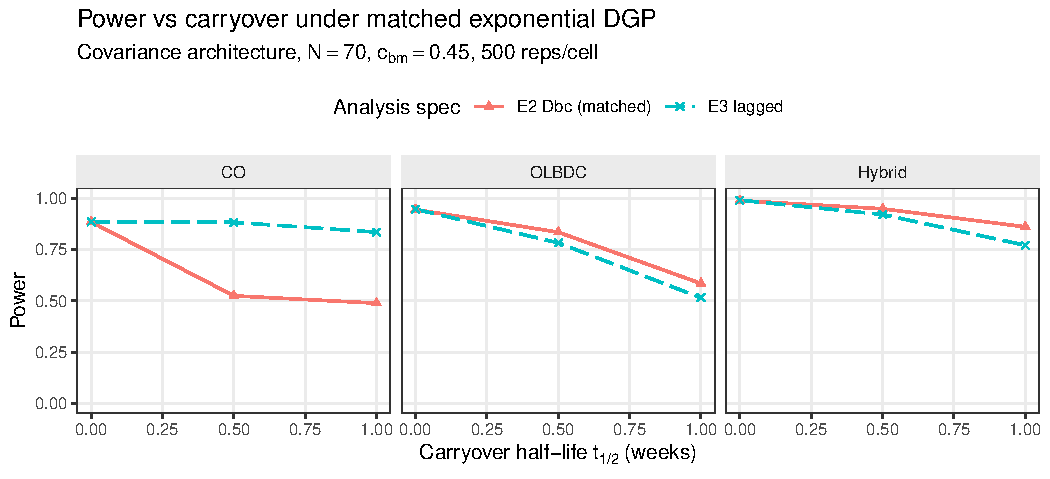
\includegraphics[width=0.95\linewidth]{../../figures/02xs-power-by-spec} \caption{Power versus carryover half-life under the exponential DGP, Architecture B, stratified by analysis specification. M2 retains a modest advantage over M3 in the Hybrid and OL+BDC designs at $t_{1/2} = 1.0$ weeks, but is dominated by M3 under the crossover (CO) design.}\label{fig:fig-power-by-spec}
\end{figure}

\begin{bullets}

\textbf{The two specifications coincide at zero carryover and diverge
as it grows, but M2's lead is confined to the two non-crossover
designs.}

\begin{itemize}\setlength{\itemsep}{2pt}\setlength{\parskip}{0pt}
\item Both are near-identical at $t_{1/2} = 0$.
\item M2's advantage emerges at $t_{1/2} = 0.5$ and grows in the
Hybrid and OL+BDC designs.
\item Under the CO design M2 is dominated by M3 (Section 5).
\end{itemize}

\end{bullets}

\begin{rgt}
rgt to complete.

\end{rgt}

\begin{orig}
The two analysis specifications yield near-identical power at
\(t_{1/2} = 0\), where there is no carryover to model, and diverge
progressively as carryover half-life increases. M2 retains a modest
but consistent advantage in the Hybrid and OL+BDC designs, where the
advantage emerges at \(t_{1/2} = 0.5\) weeks and grows through
\(t_{1/2} = 1.0\) weeks. This advantage does not appear under the
crossover (CO) design, where M2 is in fact dominated (Section 5): in
a crossover the within-subject correlation already carries most of
the signal M2's decaying predictor is designed to recover, so M2 has
nothing left to gain and its down-weighting of off-drug points only
hurts.

\end{orig}

\subsection{Decay-form mis-specification}\label{decay-form-mis-specification}

\begin{figure}
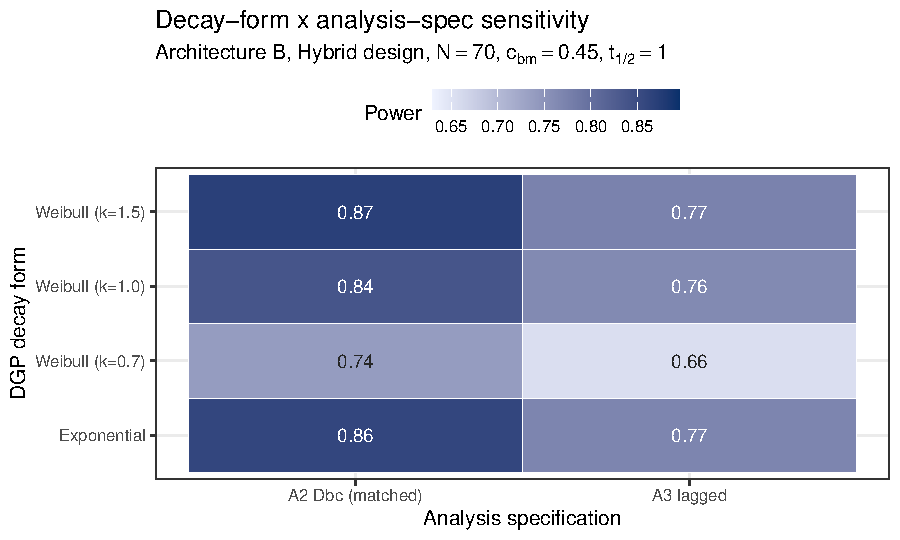
\includegraphics[width=0.7\linewidth]{../../figures/02xs-heatmap-matched-vs-mismatched} \caption{Power at the critical cell ($t_{1/2} = 1.0$ weeks, Architecture B, Hybrid design, $N = 70$, $c_{bm} = 0.45$) across DGP decay forms (rows) and analysis specifications (columns). Under the heavy-tailed Weibull DGP ($k = 0.7$), M2's advantage over M3 narrows because its assumed exponential decay no longer matches truth. The fill scale is stretched to the observed power range (0.66-0.87), not the full [0,1] range, so that these cell-to-cell differences are visible; the absolute shading should not be compared to other figures in this manuscript.}\label{fig:fig-heatmap-mismatch}
\end{figure}

\begin{bullets}

\textbf{The heatmap separates two mis-specification directions:
wrong analysis given the DGP, and wrong assumed DGP.}

\begin{itemize}\setlength{\itemsep}{2pt}\setlength{\parskip}{0pt}
\item Matched reference (exp DGP $\times$ M2): power
$0.860 \pm 0.016$.
\item Same row, M3 column: penalty of the lagged specification under
an exponential DGP.
\item M2 column, other rows: cost of assuming exponential when the
truth is Weibull.
\end{itemize}

\end{bullets}

\begin{rgt}
rgt to complete.

\end{rgt}

\begin{orig}
The heatmap cell at the intersection of the exponential DGP row and
the M2 analysis column is the matched reference
(power \(0.860 \pm 0.016\)). The same row's M3 column quantifies the
power penalty of the lagged specification when the DGP is
exponential; the M2 column's other rows quantify the cost of
assuming exponential decay in the analysis when the true DGP is
Weibull. Even under the heaviest-tailed Weibull DGP (\(k = 0.7\)), M2's
advantage over M3 narrows but does not reverse; the Discussion
(Section 5) takes up the practical interpretation.

\end{orig}

\subsection{Type I error control and cluster-robust recalibration}\label{type-i-error-control-and-cluster-robust-recalibration}

\begin{figure}
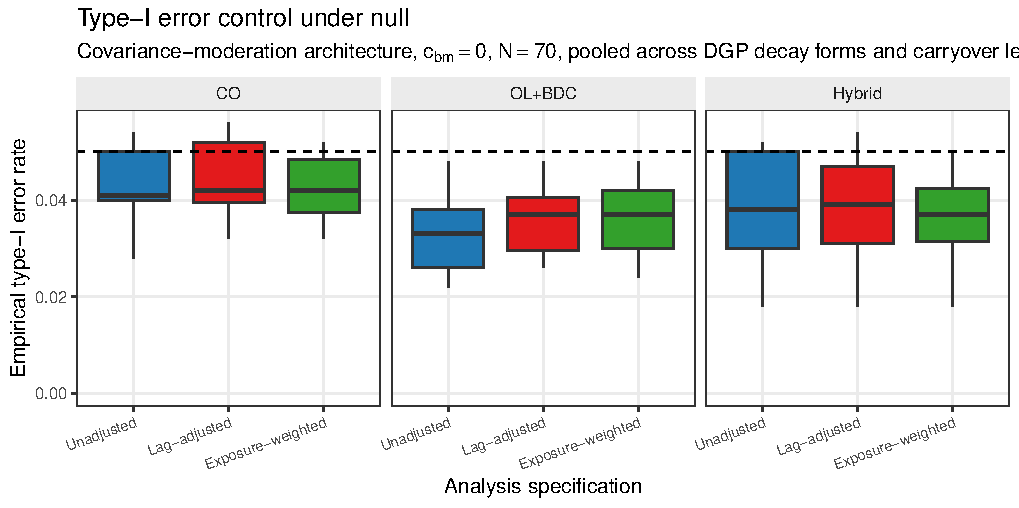
\includegraphics[width=0.8\linewidth]{../../figures/02xs-type1-boxplots} \caption{Empirical Type I error rates under the null ($c_{bm} = 0$), Architecture B, pooled across DGP decay forms and carryover half-lives, stratified by design and analysis specification. Boxplots cover the distribution across cells at $N = 70$; the dashed reference line marks the nominal 0.05 level.}\label{fig:fig-type1}
\end{figure}

\begin{bullets}

\textbf{Type I error is conservative, reflecting the corCAR1
working-covariance conservatism rather than inflation.}

\begin{itemize}\setlength{\itemsep}{2pt}\setlength{\parskip}{0pt}
\item Neither specification inflates the rate above nominal in any
design.
\item The companion calibration study traces the shortfall to a
6-10\% over-estimated SE.
\item Block S6's CR2 (below) restores nominal size without changing
the ranking.
\end{itemize}

\end{bullets}

\begin{rgt}
rgt to complete.

\end{rgt}

\begin{orig}
Across the null cells, empirical Type I error is uniformly below the
nominal 0.05 level for both specifications and all three designs.
That shortfall is not sampling slack but the conservatism of the
model-based interaction test that the companion calibration study\textsuperscript{\citeproc{ref-pmsimstats_calibration2026}{5}} traces to the corCAR1 working
covariance: its standard error is over-estimated by six to ten
percent and the realized rejection rate falls correspondingly. The
conservatism is uniform across specifications, which is why it
leaves the comparison intact; the cluster-robust recalibration
reported below (block S6) confirms that a CR2 cluster-robust standard
error restores the rejection rate to nominal without disturbing the
ranking. Table \ref{tab:tab-type1-cr2} makes the per-specification
conservatism and its cluster-robust correction explicit at the null
cell.

\end{orig}

\begin{table}

\caption{\label{tab:tab-type1-cr2}Conservatism of the model-based interaction test and its
    cluster-robust correction, at the null cell ($c_{bm} = 0$,
    exponential DGP, $t_{1/2} = 1.0$ weeks, Hybrid design, $N = 70$,
    Architecture B, 3{,}000 replicates). $\kappa$ is the ratio of the
    mean standard error to the empirical standard deviation of the
    interaction estimate; $\kappa > 1$ indicates a conservative
    test. Both specifications are conservative under the model-based
    test, most so the exposure-weighted M2 ($\kappa = 1.10$, Type I
    $= 0.029$); the CR2 bias-reduced cluster-robust standard error
    restores $\kappa$ to near one and Type I to nominal (0.045 to
    0.049) for both specifications.}
\centering
\begin{tabular}[t]{lllll}
\toprule
Specification & $\kappa$ model & Type I model & $\kappa$ CR2 & Type I CR2\\
\midrule
M2 & 1.10 & 0.029 & 1.00 & 0.045\\
M3 & 1.05 & 0.039 & 0.98 & 0.049\\
\bottomrule
\end{tabular}
\end{table}

\begin{table}
\centering
\caption{\label{tab:tab-s6}Cluster-robust recalibration of M2 (Power columns) and
    of the M2$-$M3 ranking (last two columns), at the reference cell
    and four stress cells (500 replicates, $c_{bm} = 0.45$,
    Architecture B). $\kappa$ is the ratio of the mean standard
    error to the empirical standard deviation of the interaction
    estimate for M2; a value above one is a conservative test. The
    M2$-$M3 columns are computed directly from the per-specification
    power at this cell under each inference, so they are a genuine
    check of this manuscript's own comparison rather than the
    M2-vs-M1 contrast reported for the full-scope grid. CR2 df is
    the mean Satterthwaite degrees of freedom for the cluster-robust
    test on M2. Computed with \texttt{clubSandwich}.}
\centering
\resizebox{\ifdim\width>\linewidth\linewidth\else\width\fi}{!}{
\begin{tabular}[t]{llllllll}
\toprule
Cell & $\kappa$ model & $\kappa$ CR2 & Power model & Power CR2 & M2$-$M3 model & M2$-$M3 CR2 & CR2 df\\
\midrule
Reference, $N=70$ & 1.15 & 0.99 & 0.829 & 0.863 & +0.082 & +0.090 & 23\\
Small $N=35$ & 1.13 & 0.96 & 0.558 & 0.590 & +0.068 & +0.086 & 12\\
High autocorr, $\rho=0.9$ & 1.26 & 0.94 & 0.954 & 0.980 & +0.052 & +0.036 & 23\\
Half-life mis-spec & 1.14 & 1.00 & 0.759 & 0.795 & +0.012 & +0.022 & 23\\
30\% MCAR dropout & 0.99 & 0.85 & 0.148 & 0.126 & +0.014 & -0.000 & 5\\
\bottomrule
\end{tabular}}
\end{table}

\begin{figure}
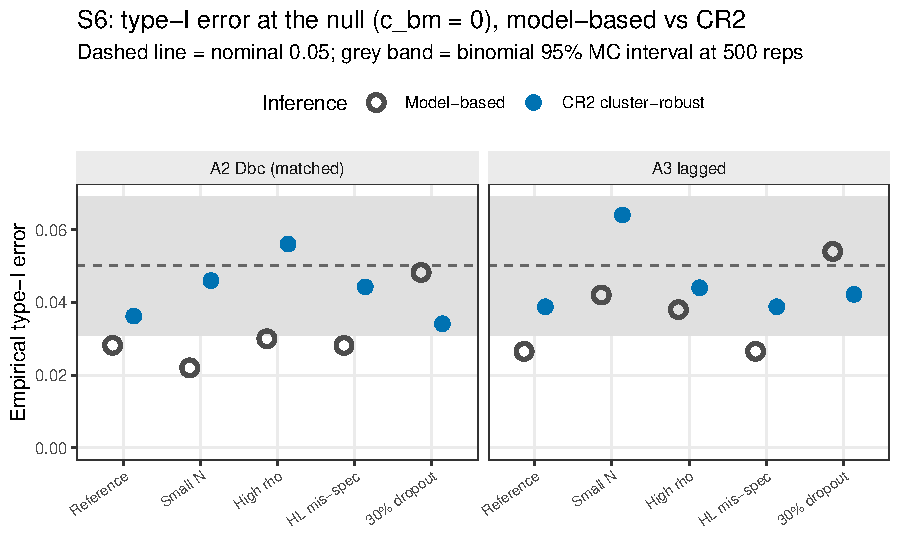
\includegraphics[width=0.8\linewidth]{../../figures/02xs-type1-cr2} \caption{Empirical Type I error at the null ($c_{bm} = 0$) under model-based and CR2 cluster-robust inference, across the five S6 stress cells and the two specifications (Architecture B). The model-based test (open) is conservative (near 0.03); CR2 (filled) is restored to the nominal 0.05 (dashed), within the binomial Monte Carlo band (gray). 500 null replicates per cell.}\label{fig:fig-type1-cr2}
\end{figure}

\begin{bullets}

\textbf{CR2 restores nominal size and recovers two to five power
points; the M2-vs-M3 ranking is held or widened at four of five S6
cells but collapses to a statistical tie under 30\% dropout.}

\begin{itemize}\setlength{\itemsep}{2pt}\setlength{\parskip}{0pt}
\item Model-based null rejection sits near 0.03-0.04 across cells and
specs; CR2 restores it to a mean near nominal.
\item $\kappa$ falls from 1.07-1.26 to about 1 under CR2 (computed
for M2; M3's calibration ratio is comparable, Table
\\ref{tab:tab-type1-cr2}).
\item The M2$-$M3 gap widens under CR2 at the reference, small-$N$,
and half-life-mis-spec cells, narrows slightly at high autocorrelation,
and is effectively zero (within noise) under 30\% dropout, consistent
with the S3 dropout finding below.
\item Validated only at Architecture B / Hybrid / $N = 70$; do not
extend the reading to the CO design.
\end{itemize}

\end{bullets}

\begin{rgt}
rgt to complete.

\end{rgt}

\begin{orig}
Figure \ref{fig:fig-type1-cr2} shows the effect of recalibration on
test size directly: the model-based null rejection rate sits below
nominal across the five S6 cells and both specifications, while the
CR2 test restores it to within the Monte Carlo band around 0.05. This
is the precondition for the whole comparison -- a test that is not
correctly sized cannot be preferred on power alone. In the
information-rich cells, the calibration ratio \(\kappa\) runs 1.07-1.26
under the model and is restored to about 1 under CR2, and the
correctly-sized test recovers two to five points of power. Table
\ref{tab:tab-s6} reports the M2\(-\)M3 gap -- this manuscript's own
comparison, computed directly from the per-specification power at
each S6 cell rather than reused from the M2-vs-M1 contrast reported
in the full-scope grid. The gap is held or slightly widened under CR2
at the reference cell (\(+0.080 \to +0.092\)), the small-\(N\) cell
(\(+0.068 \to +0.086\)), and the half-life-mis-specification cell
(\(+0.012 \to +0.022\)); it narrows somewhat under high autocorrelation
(\(+0.052 \to +0.036\), both favoring M2); and at 30\% MCAR dropout it
collapses from a small M2 lead under the model-based test (\(+0.014\))
to an essentially null difference under CR2 (\(-0.0002\)), i.e.~a
statistical tie. This is not a contradiction of the ranking so much
as a restatement of the dropout finding in block S3 below: M2's
advantage is driven by information in off-drug observations, and
once dropout has removed most of that information there is little
left for either the model-based test or its cluster-robust correction
to distinguish. This recalibration was validated only in the
Architecture\textasciitilde B, Hybrid, \(N = 70\) cells and should not be extended to
the crossover design, where M2 does not lead.

\end{orig}

\subsection{Sensitivity analyses}\label{sensitivity-analyses}

\begin{bullets}

\textbf{Four Tier 2 blocks perturb one axis at a time around the
reference cell.}

\begin{itemize}\setlength{\itemsep}{2pt}\setlength{\parskip}{0pt}
\item Reference: Architecture B, Hybrid, $N = 70$, $c_{bm} = 0.45$,
exponential DGP, $t_{1/2} = 1.0$.
\item Each block varies one axis with the others held fixed.
\item Blocks are reported separately, not pooled with Tier 1 or each
other.
\end{itemize}

\end{bullets}

\begin{rgt}
rgt to complete.

\end{rgt}

\subsubsection{S1: within-factor autocorrelation}\label{s1-within-factor-autocorrelation}

\begin{figure}
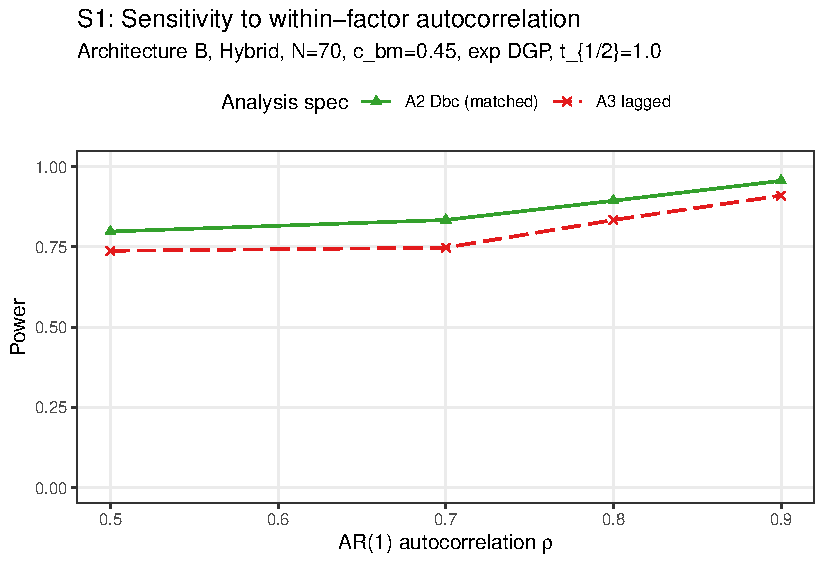
\includegraphics[width=0.6\linewidth]{../../figures/02xs-sens-S1} \caption{Power by analysis specification across AR(1) autocorrelation $\rho \in \{0.5, 0.7, 0.8, 0.9\}$, Architecture B.}\label{fig:fig-sens-s1}
\end{figure}

\begin{bullets}

\textbf{S1: autocorrelation lifts both specifications equally,
preserving M2's $\approx 0.06$ advantage at every $\rho$.}

\begin{itemize}\setlength{\itemsep}{2pt}\setlength{\parskip}{0pt}
\item Power rises monotonically with $\rho$ for both.
\item M2's advantage holds near 0.06 across $\rho \in [0.5, 0.9]$.
\item Autocorrelation and the specification act additively, not
multiplicatively.
\end{itemize}

\end{bullets}

\begin{rgt}
rgt to complete.

\end{rgt}

\begin{orig}
Both specifications gain power monotonically with \(\rho\). At
\(\rho = 0.5\), M2 power is \(0.798 \pm 0.018\) versus M3
\(0.738 \pm 0.020\); at \(\rho = 0.9\), M2 reaches \(0.956 \pm 0.009\)
versus M3 \(0.910 \pm 0.013\) (point estimate \(\pm\) MCSE,
\(n_{sim} = 500\)). The M2 advantage over M3, approximately 0.06 in
absolute power throughout, is preserved at every AR(1) level: the
interaction between autocorrelation strength and analysis
specification is additive rather than multiplicative.

\end{orig}

\subsubsection{S2: analyst-truth half-life mismatch}\label{s2-analyst-truth-half-life-mismatch}

\begin{figure}
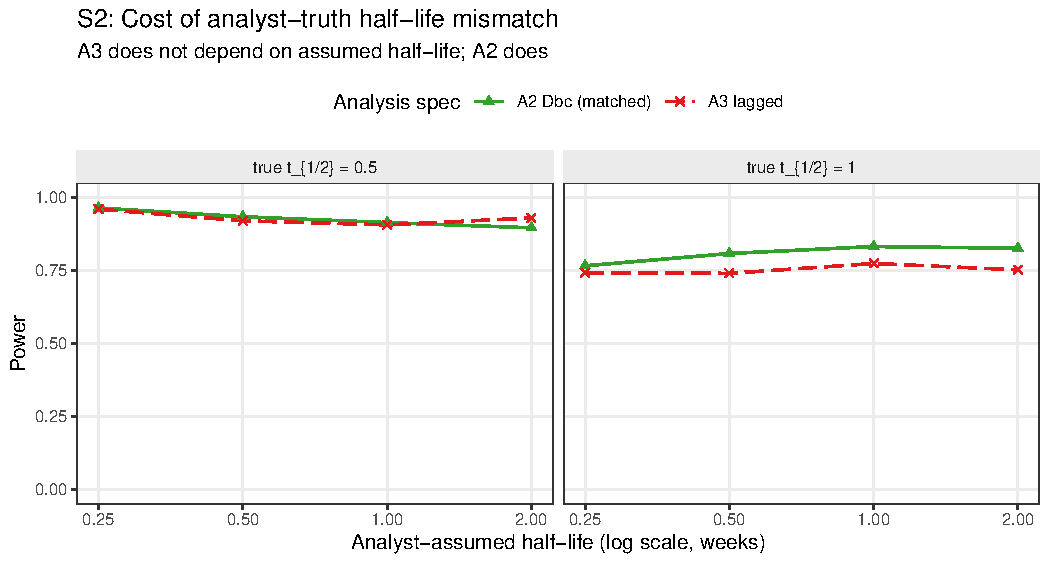
\includegraphics[width=0.8\linewidth]{../../figures/02xs-sens-S2} \caption{Power of M2 and M3 as the analyst's assumed half-life departs from the true DGP half-life. M3 is invariant to the assumed half-life by construction; M2's power degrades with mis-specification.}\label{fig:fig-sens-s2}
\end{figure}

\begin{bullets}

\textbf{S2: M2 keeps its advantage even when the assumed half-life
is wrong by a factor of two or four.}

\begin{itemize}\setlength{\itemsep}{2pt}\setlength{\parskip}{0pt}
\item M2 averages 0.868 over eight assumed/true half-life cells
(range 0.766-0.964).
\item M3 is invariant to the assumed half-life (average 0.840).
\item M2's gentle curvature makes it a defensible default under an
approximately-known half-life.
\end{itemize}

\end{bullets}

\begin{rgt}
rgt to complete.

\end{rgt}

\begin{orig}
M2 is markedly robust to analyst-truth half-life mismatch. Across the
eight S2 cells (DGP \(t_{1/2} \in \{0.5, 1.0\}\) weeks crossed with
analyst-assumed \(t_{1/2} \in \{0.25, 0.5, 1.0, 2.0\}\) weeks), M2
averages 0.868, ranging from 0.766 to 0.964; per-cell MCSE ranges
from 0.008 to 0.019. M3 is invariant to the analyst-assumed half-life
by construction, as it does not consume the parameter, and its power
averages 0.840 across the same eight cells. The exposure-weighted
predictor's curvature is sufficiently gentle that mis-specification
of the assumed half-life by a factor of two does not erode M2's
advantage over M3 at either DGP half-life, suggesting M2 remains
defensible even when the true pharmacokinetic half-life is only
approximately known at the design stage.

\end{orig}

\subsubsection{S3: dropout}\label{s3-dropout}

\begin{figure}
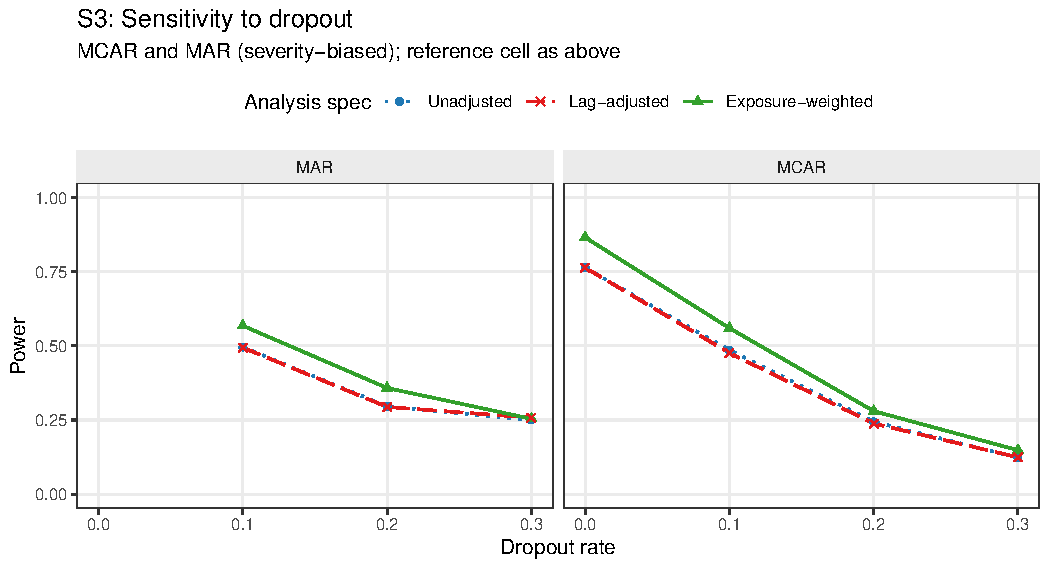
\includegraphics[width=0.8\linewidth]{../../figures/02xs-sens-S3} \caption{Power at dropout rates $\in \{0, 0.1, 0.2, 0.3\}$ under MCAR and MAR mechanisms, Architecture B.}\label{fig:fig-sens-s3}
\end{figure}

\begin{bullets}

\textbf{S3: dropout collapses power for both methods, and narrows
M2's advantage as off-drug observations are dropped.}

\begin{itemize}\setlength{\itemsep}{2pt}\setlength{\parskip}{0pt}
\item At 30\% MCAR both fall to about 0.12-0.15, effectively tied.
\item The M2$-$M3 gap shrinks from $\approx 0.10$ (no dropout) to
$\approx 0.03$ (30\% MCAR).
\item M2's signal lives in off-drug points, so dropping them erodes
its edge; the advantage survives at dropout $\leq 0.20$.
\end{itemize}

\end{bullets}

\begin{rgt}
rgt to complete.

\end{rgt}

\begin{orig}
Both specifications lose power monotonically with dropout rate. The
MCAR baseline (\(N = 70\), dropout = 0) gives M2 \(0.866 \pm 0.015\),
M3 \(0.764 \pm 0.019\); at MCAR rate 0.30 these collapse to M2
\(0.148 \pm 0.016\), M3 \(0.124 \pm 0.015\). M2's advantage narrows under
heavy dropout: the absolute M2\(-\)M3 gap is approximately 0.10 at
zero dropout, 0.07 at rate 0.10, 0.04 at rate 0.20, and 0.03 at rate
0.30 under MCAR, narrowing further under MAR at the highest rate
(\(\approx 0.004\) at rate 0.30). The pattern is consistent with M2's
signal source residing in the exposure-weighted contrast contributed
by off-drug observations: when those observations are preferentially
dropped, M2's advantage contracts toward M3's. At low-to-moderate
dropout (rate \(\leq 0.20\)) the M2 advantage is preserved.

\end{orig}

\subsubsection{S4: biomarker-moderation effect-size curve}\label{s4-biomarker-moderation-effect-size-curve}

\begin{figure}
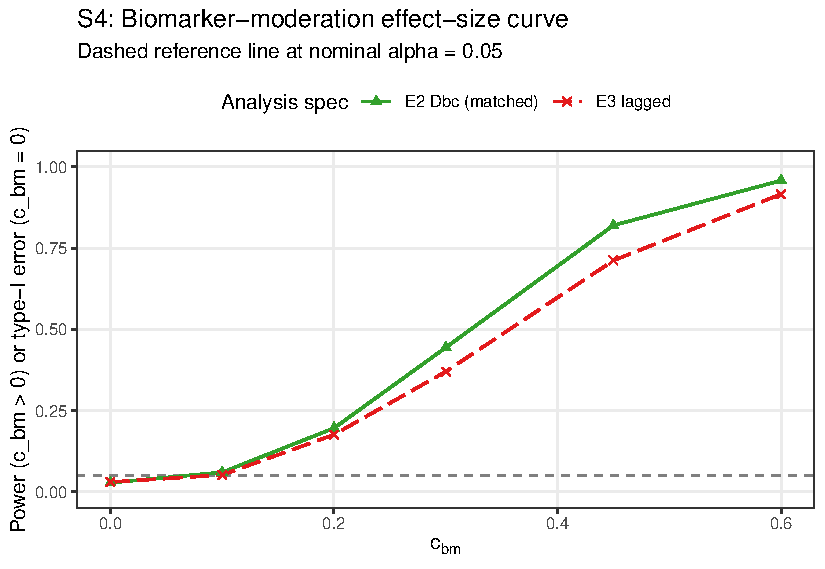
\includegraphics[width=0.6\linewidth]{../../figures/02xs-sens-S4} \caption{Power across the biomarker-moderation effect-size range $c_{bm} \in \{0, 0.10, 0.20, 0.30, 0.45, 0.60\}$ under Architecture B. The $c_{bm} = 0$ point is the null for Type I verification.}\label{fig:fig-sens-s4}
\end{figure}

\begin{bullets}

\textbf{S4: the power curve is sigmoidal; M2's advantage peaks at
intermediate effect sizes and vanishes toward the ceiling.}

\begin{itemize}\setlength{\itemsep}{2pt}\setlength{\parskip}{0pt}
\item Type I error at $c_{bm} = 0$ is conservative (0.028-0.030).
\item M2$-$M3 peaks at $+0.102$ at $c_{bm} = 0.45$, shrinking to
$+0.042$ at $c_{bm} = 0.60$.
\item The advantage matters most for moderate biomarker-treatment
interactions.
\end{itemize}

\end{bullets}

\begin{rgt}
rgt to complete.

\end{rgt}

\begin{orig}
The expected sigmoidal power curve is observed for both
specifications. At \(c_{bm} = 0\), empirical Type I error is below
nominal at \(0.028 \pm 0.007\) (M2) and \(0.030 \pm 0.008\) (M3); power
rises through the mid-range and saturates at \(c_{bm} \geq 0.45\): at
\(c_{bm} = 0.6\), M2 reaches \(0.958 \pm 0.009\) and M3
\(0.916 \pm 0.012\). The M2 advantage is largest at intermediate effect
sizes, \(+0.082\) absolute at \(c_{bm} = 0.30\) and \(+0.102\) at
\(c_{bm} = 0.45\), shrinking to \(+0.042\) at \(c_{bm} = 0.60\) where both
specifications approach ceiling. The advantage is therefore most
practically consequential in designs targeting moderate
biomarker-treatment interactions.

\end{orig}

\subsection{A higher-precision check}\label{a-higher-precision-check}

\begin{bullets}

\textbf{A high-precision paired-McNemar rerun finds M2 strictly ahead
of M3 only at the highest-leverage cell ($+7.2$ points,
$p = 1.2 \times 10^{-7}$); elsewhere the two are operationally tied.}

\begin{itemize}\setlength{\itemsep}{2pt}\setlength{\parskip}{0pt}
\item 24-cell OL+BDC rerun at 600 trials/cell, all converging.
\item Paired McNemar (same trials): M2 beats M3 by 7.2 points at
$N = 70$, $t_{1/2} = 1.0$; other three cells show
$|\Delta| \leq 1.5$ points, $p \geq 0.18$.
\item Type I error across the null cells stayed in $[0.003, 0.053]$.
\end{itemize}

\end{bullets}

\begin{rgt}
rgt to complete.

\end{rgt}

\begin{orig}
Because some Tier 1 gaps are small, a focused 24-cell grid (the
OL+BDC design, \(N \in \{35, 70\}\), true half-life
\(\in \{0.5, 1.0\}\)) was rerun at 600 trials per cell, all converging;
because M2 and M3 see the \emph{same} trials, they can be compared with a
paired \textbf{McNemar test}, more sensitive than treating the
specifications as independent. Type I error across the twelve null
cells fell in \([0.003, 0.053]\), so both specifications hold nominal
alpha at the explored \(N\) and DGP half-life combinations. Paired
McNemar on M2 versus M3 finds M2 strictly dominant only at the
high-leverage corner (\(N = 70\), \(t_{1/2}^{\text{DGP}} = 1.0\) weeks,
\(\Delta = +7.2\) percentage points, \(p = 1.2 \times 10^{-7}\)); in the
other three cells the paired difference lies between \(-0.5\) and
\(+1.5\) percentage points with McNemar \(p \geq 0.18\), and the two
specifications are operationally tied at this resolution. Resolving
the M2-versus-M3 gap at the intermediate cells with statistical
clarity would require approximately 2\{,\}000 replicates per cell at
the current MCSE.

\end{orig}

\section{Discussion}\label{discussion}

\subsection{The main result, and where it breaks down}\label{the-main-result-and-where-it-breaks-down}

\begin{bullets}

\textbf{M2's advantage over M3 is real but conditional: confined to
the Hybrid and OL+BDC designs, and reversed under the crossover
design.}

\begin{itemize}\setlength{\itemsep}{2pt}\setlength{\parskip}{0pt}
\item Best cell (Hybrid): M2 beats M3 by $\approx 10$ points
($\approx 5$ MCSEs).
\item Under CO, M2 is much worse (0.488 vs 0.830 for M3).
\item Mechanism: the crossover's within-subject correlation already
carries the signal M2 targets, so M2 only loses there.
\end{itemize}

\end{bullets}

\begin{rgt}
rgt to complete.

\end{rgt}

\begin{orig}
The headline is that M2's advantage over M3 is real but
\textbf{conditional}. At its best cell (Hybrid design, \(N = 70\),
\(c_{bm} = 0.45\), \(t_{1/2} = 1.0\)) M2 beats M3 by about 10 percentage
points of power (0.860 vs 0.770) -- about five MCSEs, so not luck.
In the crossover design it is much \emph{worse} (0.488 vs 0.830 for M3).
There is a clean reason for the crossover failure: in a crossover the
within-subject correlation already carries most of the signal that
M2's decaying predictor is designed to recover, so M2 has nothing
left to gain and its down-weighting of off-drug points only hurts.
The ranking ``M2 best'' therefore holds only in the two non-crossover
designs studied here.

\end{orig}

\subsection{What the robustness checks add}\label{what-the-robustness-checks-add}

\begin{bullets}

\textbf{Where M2 leads, the lead survives all three robustness
checks.}

\begin{itemize}\setlength{\itemsep}{2pt}\setlength{\parskip}{0pt}
\item Decay shape: M2 never drops below M3 even when the assumed
form is wrong, up to the heaviest-tailed Weibull.
\item Assumed half-life: a two- to four-fold error moves M2 only
from 0.83 to 0.77, never below M3.
\item Autocorrelation: lifts both equally, so M2's 5-6 point lead is
$\rho$-independent.
\end{itemize}

\end{bullets}

\begin{rgt}
rgt to complete.

\end{rgt}

\begin{orig}
Three checks probe whether M2's win, where it exists, is fragile.
\textbf{Decay shape (Fig. \ref{fig:fig-heatmap-mismatch}).} Even when the
analyst wrongly assumes exponential decay but the truth is Weibull,
M2 still does not drop below M3, within the decay-shape range tested
here. \textbf{Assumed half-life (Fig. \ref{fig:fig-sens-s2}).} M3 does
not use a half-life, so it is unaffected; M2 does, yet getting the
half-life wrong by a factor of two or four moves its power only from
about 0.83 to 0.77, never below M3. \textbf{Autocorrelation
(Fig. \ref{fig:fig-sens-s1}).} Stronger serial correlation raises
both methods by about the same amount, so M2's lead stays near 5-6
points regardless of correlation strength.

\end{orig}

\subsection{Dropout matters more than the method}\label{dropout-matters-more-than-the-method}

\begin{bullets}

\textbf{Dropout collapses power for both methods equally, so it
dominates the specification choice.}

\begin{itemize}\setlength{\itemsep}{2pt}\setlength{\parskip}{0pt}
\item At 30\% dropout both fall to 0.12-0.25 and become
indistinguishable.
\item MAR (severity-related) dropout is slightly worse than MCAR,
because the highest-signal patients leave first.
\item Keeping patients in the trial buys more power than the choice
between M2 and M3.
\end{itemize}

\end{bullets}

\begin{rgt}
rgt to complete.

\end{rgt}

\begin{orig}
The most sobering result is about \emph{missing data}, not carryover.
When patients drop out (Fig. \ref{fig:fig-sens-s3}), power collapses
for both methods together: at 30\% dropout both fall to 0.12-0.25 and
become indistinguishable. M2 cannot protect against the loss; it only
organizes whatever data remain. Dropout related to severity (MAR) is
slightly worse than purely random dropout (MCAR), because the
sickest patients -- who carry the most signal -- leave first. The
practical message is blunt: keeping patients in the trial buys far
more power than the choice between M2 and M3.

\end{orig}

\subsection{Scope, related work, and limits}\label{scope-related-work-and-limits}

\begin{bullets}

\textbf{This manuscript is a narrowed slice of the full-scope grid;
its ranking should not be extrapolated to Architecture A, the binary
specification M1, or linear decay without consulting the full-scope
manuscript.}

\begin{itemize}\setlength{\itemsep}{2pt}\setlength{\parskip}{0pt}
\item Full grid (report.Rmd / report-slim.Rmd) shows M2's advantage
does not extend to Architecture A, where M2 is marginally dominated
throughout.
\item M2 power 0.860 reproduces Hendrickson's 0.82; the Jones-Kenward
expectation that shape-free M3 beats M2 under mis-specification is
not supported here.
\item Two further limitations: a single parameter set, and
one-factor-at-a-time sensitivity checks.
\end{itemize}

\end{bullets}

\begin{rgt}
rgt to complete.

\end{rgt}

\begin{orig}
This manuscript deliberately narrows the full-scope grid to
Architecture B, non-linear decay, and the M2/M3 contrast, to bring a
30-page evaluation down to a size a reviewer can read at one sitting.
The full-scope companion (report.Rmd / report-slim.Rmd) shows that
the M2 advantage documented here does not extend to Architecture A
(direct mean moderation), where M2 is marginally dominated in every
design, nor is the binary on-drug specification M1 dominated by M2
outside the Hybrid/OL+BDC-under-Architecture-B cells studied here;
readers who need the cross-architecture or M1 comparison should
consult that manuscript rather than extrapolate from this one. Within
the narrower scope, our matched-decay (M2) power at the headline
cell, \(0.860 \pm 0.016\), reproduces Hendrickson's\textsuperscript{\citeproc{ref-hendrickson2020}{2}} reported 0.82 for the same cell. The crossover
tradition of Jones and Kenward\textsuperscript{\citeproc{ref-jones2014crossover}{4}} predicted that
a shape-free lagged term (M3) should beat a parametric predictor (M2)
when the decay shape is guessed wrong; our S2 result does not support
this in the range we tested, because M2's penalty for a wrong
half-life is too small for M3 to overtake it. Two further
limitations bound these conclusions. First, the numbers come from one
parameter set (calibrated to a prazosin/PTSD trajectory), so the
\emph{absolute} power values are illustrative; the \emph{ranking} is the
portable part, and even it is conditional on the design as shown
above. Second, the sensitivity checks vary one factor at a time, so
they can miss interactions between factors (for example, high
autocorrelation combined with heavy dropout); the one joint check
reported in the full-scope manuscript (block S5) showed no
surprises.

\end{orig}

\section{Conclusions}\label{conclusions}

\begin{enumerate}
\def\labelenumi{\arabic{enumi}.}
\item
  \textbf{M2 helps, but only conditionally.} The exposure-weighted
  predictor gives the highest power -- about 10 points over M3 --
  \emph{only} in the Hybrid and OL+BDC designs, and the lead survives
  wrong decay-shape and wrong half-life assumptions there. Under
  the crossover design M2 has no advantage and M3 is at least as
  good. Where M2 is used, report it with a CR2 cluster-robust
  standard error (Block S6).
\item
  \textbf{A guessed half-life is fine (where M2 is used).} Getting the
  half-life wrong by a factor of two to four barely moves M2's
  power, so a rough pharmacokinetic estimate suffices.
\item
  \textbf{Dropout beats everything.} Power falls sharply as dropout
  rises (about half lost at 20\% dropout), the same for both
  methods. Preventing dropout matters more than the choice between
  M2 and M3.
\item
  \textbf{The test is slightly conservative, and fixable.} Both methods
  reject a little less than the nominal 5\% under the null; the CR2
  cluster-robust standard error restores the correct rate while
  recovering a few points of power. The M2-vs-M3 gap is held or
  widened under CR2 at four of the five S6 stress cells, but
  collapses to a statistical tie under 30\% dropout, consistent with
  finding 3 above (Block S6).
\item
  \textbf{This is a narrowed slice.} Architecture A, the binary
  specification M1, and linear decay are outside this manuscript's
  scope; the full-scope grid in report.Rmd / report-slim.Rmd is the
  authority for those comparisons and should be consulted before
  generalizing beyond Architecture B.
\end{enumerate}

\section*{Notes and reproducibility}\label{notes-and-reproducibility}
\addcontentsline{toc}{section}{Notes and reproducibility}

The authors declare no conflicts of interest and received no
specific funding. This manuscript is a scope-narrowed derivative of
report-slim.Rmd: it re-filters, but does not re-run, the same
production simulation. Cell-level summaries are at
\texttt{analysis/data/02-grid-summary.rds} and
\texttt{02-sensitivity-summary.rds}; filtered figures are produced by
\texttt{03-render-figures-extra-slim.R}, \texttt{04-sensitivity-figures-extra-slim.R},
and \texttt{07-type1-cr2-figure-extra-slim.R} under
\texttt{analysis/scripts/carryover-sensitivity/}. No simulation runs during
knitting. The production simulation ran under R 4.5.3 and the
document is rendered under R 4.6.0, both pinned via \texttt{renv.lock}.

\section{References}\label{references}

\protect\phantomsection\label{refs}
\begin{CSLReferences}{0}{1}
\bibitem[\citeproctext]{ref-morris2019simulation}
\CSLLeftMargin{1. }%
\CSLRightInline{Morris TP, White IR, Crowther MJ. Using simulation studies to evaluate statistical methods. \emph{Statistics in Medicine}. 2019;38(11):2074-2102. doi:\href{https://doi.org/10.1002/sim.8086}{10.1002/sim.8086}}

\bibitem[\citeproctext]{ref-hendrickson2020}
\CSLLeftMargin{2. }%
\CSLRightInline{Hendrickson RC, Thomas RG, Schork NJ, Raskind MA. Optimizing aggregated {N}-of-1 trial designs for predictive biomarker validation: Statistical methods and practical considerations. \emph{Frontiers in Digital Health}. 2020;2:13. doi:\href{https://doi.org/10.3389/fdgth.2020.00013}{10.3389/fdgth.2020.00013}}

\bibitem[\citeproctext]{ref-pmsimstats_dgp_architectures2026}
\CSLLeftMargin{3. }%
\CSLRightInline{{pmsimstats team}. Two architectures for simulating biomarker-treatment interactions in aggregated {N}-of-1 trials. Published online 2026.}

\bibitem[\citeproctext]{ref-jones2014crossover}
\CSLLeftMargin{4. }%
\CSLRightInline{Jones B, Kenward MG. \emph{Design and Analysis of Cross-over Trials}. 3rd ed. CRC Press; 2014.}

\bibitem[\citeproctext]{ref-pmsimstats_calibration2026}
\CSLLeftMargin{5. }%
\CSLRightInline{{pmsimstats team}. Type-{I} calibration of fixed-effect interaction tests in linear mixed models: A staged diagnosis of working-covariance mis-specification and a cluster-robust remedy. Published online 2026.}

\end{CSLReferences}

\vfill

\begin{center}\rule{0.5\linewidth}{0.5pt}\end{center}

\emph{Rendered on 2026-07-30 at 14:06 PDT.}\\
\emph{Source: \texttt{\textasciitilde{}/prj/res/36-pmsimstats-ng/pmsimstats-ng/analysis/report/02-carryover-sensitivity/report-extra-slim.Rmd}}

\end{document}
